\begin{name}
	{ÔN TẬP KIỂM TRA GIỮA HỌC KÌ 1}
	{TOÁN 10}
	{LỚP TOÁN THẦY PHÁT}
	{\thoigian}
\end{name}

\caulc

\Opensolutionfile{ans}[ans-ABCD]

\begin{ex}%[0D1N1-1]%[KNTT - Lớp 10 - Ôn tập giữa học kì 1 - Đề 1]%[Dương Văn Đức]
	Trong các câu sau, câu nào là mệnh đề Toán học?
	\def\dotEX{}
	\choice
	{$x^2-2x-3=0$.}
	{Bây giờ là 8 giờ sáng.}
	{\True $x=3$ là nghiệm phương trình $x^2-3=0$.}
	{Gia nhập Sát quỷ đoàn đi Akaza.}
	\loigiai{
		\lq\lq$x=3$ là nghiệm phương trình $x^2-3=0$\rq\rq~ là mệnh đề sai.
	}
\end{ex}

\begin{ex}%[0D1N1-2]%[KNTT - Lớp 10 - Ôn tập giữa học kì 1 - Đề 1]%[Dương Văn Đức]
	Mệnh đề nào sau đây là mệnh đề \textbf{sai}?
	\choice
	{\True \lq\lq $\forall x\in \mathbb{R}\colon x^2>0$\rq\rq}
	{\lq\lq $\exists n\in \mathbb{N}\colon n=n^2$\rq\rq}
	{\lq\lq $\exists n\in \mathbb{N}\colon n\leq 2n$\rq\rq}
	{\lq\lq $\exists x\in \mathbb{R}\colon x>x^2$\rq\rq}
	\loigiai{
		\begin{itemize}
			\item Ta có $x^2\geq 0$, $\forall x\in \mathbb{R}\Rightarrow$ mệnh đề \lq\lq $\forall x\in \mathbb{R}\colon x^2>0$\rq\rq~ sai.
			\item \lq\lq $\exists n\in \mathbb{N}:n=n^2$\rq\rq~ đúng vì tồn tại $n=1$ thỏa mãn.
			\item  \lq\lq $\exists n\in \mathbb{N}\colon n\leq 2n$\rq\rq~ đúng vì tồn tại $n=1$ thỏa mãn.
			\item  \lq\lq $\exists x\in \mathbb{R}\colon x>x^2$\rq\rq~ đúng vì tồn tại $x=\dfrac{1}{2}$ thỏa mãn.
		\end{itemize}
	}
\end{ex}

\begin{ex}%[0D1N1-4]%[KNTT - Lớp 10 - Ôn tập giữa học kì 1 - Đề 1]%[Dương Văn Đức]
	Cho mệnh đề $P\colon$ \lq\lq Nếu $a$ và $b$ chia hết cho $3$ thì $a+b$ cũng chia hết cho $3$\rq\rq. Mệnh đề nào là mệnh đề đảo của mệnh đề $P$?
	\choice
	{Nếu $a+b$ chia hết cho $3$ thì $a$ chia hết cho $3$}
	{Nếu $a+b$ chia hết cho $3$ thì $b$ chia hết cho $3$}
	{Nếu $a$ và $b$ không chia hết cho $3$ thì $a+b$ cũng không chia hết cho $3$}
	{\True Nếu $a+b$ chia hết cho $3$ thì $a$ và $b$ chia hết cho $3$}
	\loigiai{
		Mệnh đề đảo của mệnh đề $P$ là
		\lq\lq Nếu $a+b$ chia hết cho $3$ thì $a$ và $b$ chia hết cho $3$\rq\rq.
	}
\end{ex}

\begin{ex}%[0D1N2-3]%[KNTT - Lớp 10 - Ôn tập giữa học kì 1 - Đề 1]%[Dương Văn Đức]
	Hình vẽ dưới biểu diễn cho tập hợp nào trên trục số?
	\begin{center}
		\begin{tikzpicture}[>=stealth,declare function={a=-1;b=2;}]
			\path[pattern=north east lines] (-3,-2pt) rectangle (4.9,2pt);
			\begin{scope}
				\clip (a,-2pt) rectangle (b,2pt);
				\fill[white] (a,-3pt) rectangle (b,3pt);
			\end{scope}
			\draw[->](-3,0)->(5,0);
			\path (a,0)node{$\big ($}node[below=1ex]{$-2$}
			(b,0)node{$\big ]$}node[below=1ex]{$3$};
		\end{tikzpicture}
	\end{center}
	\choice
	{$[-2;3]$}
	{\True $(-2;3]$}
	{$[-2;3)$}
	{$(-2;3)$}
	\loigiai{
		Hình vẽ trên biểu diễn tập hợp $(-2;3]$.
	}
\end{ex}

\begin{ex}%[0D1N3-2]%[KNTT - Lớp 10 - Ôn tập giữa học kì 1 - Đề 1]%[Dương Văn Đức]
	Cho hai tập hợp $A=\{1;2;5;6\}$, $B=\{1;2;3;4;5;6;7;8\}$ khi đó tập $C_BA$ là
	\choice
	{$\{1;2;4;6\}$}
	{$\{4;6\}$}
	{\True $\{3;4;7;8\}$}
	{$\{2;6;7;8\}$}
	\loigiai{
		Tất cả các phần tử có trong tập $B$ và không thuộc tập $A$ là $C_BA=\{3;4;7;8\}$.
	}
\end{ex}
\begin{ex}
	Cho $x\in\left(90^\circ;180^\circ\right)$. Phát biểu nào sau đây là đúng?
	\choice
	{\True $\sin x>0$}
	{$\cos x>0$}
	{$\tan x>0$}
	{$\cot x>0$}
	\loigiai{
		Khi $x\in\left(90^\circ;180^\circ\right)$ thì $\sin x>0$, $\cos x<0$, $\tan x<0$, $\cot x<0$.
	}
\end{ex}

\begin{ex}
	Cho góc $a$ thoả $0^\circ \le a \le 180^\circ$. Trong các mệnh đề sau, mệnh đề nào đúng?
	\choice
	{$\sin a = \sin (180^\circ - a)$}
	{\True $\cos a = -\cos (180^\circ - a)$}
	{$\tan a = \tan (180^\circ - a)$}
	{$\cot a = \cot (180^\circ - a)$}
	\loigiai{
		Khi $0^\circ \le a \le 180^\circ$ thì $\sin a = \sin (180^\circ - a)$, $\cos a = -\cos (180^\circ - a)$, $\tan a = -\tan (180^\circ - a)$, $\cot a = -\cot (180^\circ - a)$.
	}
\end{ex}

\begin{ex}%[0H4N2-1]%[CD-Lớp 10-Ôn tập cuối học kì 1-Đề 5]%[Hoàng Ngọc Lâm]
	Cho tam giác $A B C$ với $B C=a, A C=b, A B=c$. Đẳng thức nào đúng?
	\choice
	{$a^2=b^2+c^2+2 b c \cos A$}
	{\True $a^2=b^2+c^2-2 b c \cos A$}
	{$a^2=b^2+c^2-2 b c \cos C$}
	{$a^2=b^2+c^2-2 b c \cos B$}
	\loigiai{
		Theo định lý cosin trong tam giác $A B C$, ta có $a^2=b^2+c^2-2 b c \cos A$.
	}
\end{ex}

\begin{ex}%[0H4H2-2]%[KNTT - Lớp 10 - Ôn tập giữa học kì 1 - Đề 1]%[Dương Văn Đức]
	Cho tam giác $ABC$ có $AB=c$, $AC=b$ và góc $A$. Diện tích $S$ của tam giác $ABC$ được tính theo công thức nào sau đây?
	\choice
	{$S=bc\sin A$}
	{$S=\dfrac{1}{2}bc\cos A$}
	{$S=bc\cos A$}
	{\True $S=\dfrac{1}{2}bc\sin A$}
	\loigiai{
		Ta có $S=\dfrac{1}{2}bc\sin A$.
	}
\end{ex}

\begin{ex}%[0D2H1-2]%[KNTT - Lớp 10 - Ôn tập giữa học kì 1 - Đề 1]%[Dương Văn Đức]
	Cho bất phương trình $2x-y\leq 3$. Miền nghiệm của bất phương trình trong mặt phẳng tọa độ $Oxy$ là
	\choice
	{Nửa mặt phẳng chứa điểm $O$ có bờ là đường thẳng $2x-y+3=0$}
	{Nửa mặt phẳng không chứa điểm $O$ có bờ là đường thẳng $2x-y+3=0$}
	{\True Nửa mặt phẳng chứa điểm $O$ có bờ là đường thẳng $2x-y=3$}
	{Nửa mặt phẳng không chứa điểm $O$ có bờ là đường thẳng $2x-y=3$}
	\loigiai{
		Vì $2\cdot 0 - 0 <3$ nên miền nghiệm của bất phương trình $2x-y\leq 3$ là nửa mặt phẳng chứa điểm $O$ có bờ là đường thẳng $2x-y=3$.
	}
\end{ex}
\begin{ex}%[0D2H1-2]%[Đề cương Nguyễn Hiền]%[Mui Doan,DA4-ĐC-NTH-T10]
	Đường thẳng $\Delta$ chia mặt phẳng toạ độ $Oxy$ làm hai miền. Miền không gạch sọc (không kể biên) ở hình vẽ dưới đây là miền nghiệm của bất phương trình nào?
	\begin{center}
		\begin{tikzpicture}
			\foreach \x/\y/\t in {0/0/O,-2.5/-.5/A, -2.5/4/B, 2/4/C}{
					\path (\x,\y) coordinate (\t);
				}
			\draw[->] (-2.5,0)--(2.2,0) node[below right] {$x$};
			\draw[->] (0,-1.3)--(0,4) node[right] {$y$};
			\node (0,0) [below right]{$ O $};
			\foreach \x in {-2,-1,1,2}
			\draw[shift={(\x,0)},color=black] (0pt,2pt) -- (0pt,-2pt);
			\foreach \y in {-1,1,2,3}
			\draw[shift={(0,\y)},color=black] (2pt,0pt) -- (-2pt,0pt);
			\draw (0,2)node[below right]{$2$} (-2,0)node[below right]{$-2$}
			(1,2.8)node[below]{$\Delta$}
			;
			\draw [domain=-2.5:2, samples=100] plot (\x, {(1) * \x +2});
			\fill (0,0) circle (1pt) ;
			\draw[pattern=north east lines] (A)--(B)--(C);
		\end{tikzpicture}
	\end{center}
	\choice
	{$x+y+2\geq 0$}
	{$x-y+2\leq 0$}
	{\True $x-y+2> 0$}
	{$x-2y+2> 0$}
	\loigiai{
		Đường thẳng $\Delta$ đi qua hai	điểm $(-2;0)$ và $(0;2)$ nên $\Delta\colon y=x+2\Leftrightarrow x-y+2=0$.\\
		Điểm $O(0;0)$ nằm trong miền nghiệm và $0-0+2=2>0$ nên phần không gạch sọc là miền nghiệm của bất phương trình $x-y+2> 0$.
	}
\end{ex}

\begin{ex}%[0D2H1-2]%[KNTT - Lớp 10 - Ôn tập giữa học kì 1 - Đề 1]%[Dương Văn Đức]
	Cặp số $(x;y)$ nào sau đây là nghiệm của hệ bất phương trình $\heva{&2x+3y-1>0\\&5x-y+4\leq 0}$ là
	\choice
	{$(0;0)$}
	{$(-2;-4)$}
	{$(-3;-4)$}
	{\True $(0;4)$}
	\loigiai{
		Thay lần lượt $(x;y)$ bởi các cặp số trong đáp án ta thấy $(0;4)$ là nghiệm của hệ bất phương trình.
	}
\end{ex}

\Closesolutionfile{ans}

\cauds

\Opensolutionfile{ans}[ans-DS]

\begin{ex}%[0D1H1-2]%[KNTT - Lớp 10 - Ôn tập giữa học kì 1 - Đề 1]%[Dương Văn Đức]
	Cho biểu thức $P(n)=3n^2+3n-6$ và tập hợp $B=\{n\in \mathbb{N} \mid P(n)=0\}$.
	\choiceTF
	{Mệnh đề \lq\lq $P(4)+1$ là số nguyên tố \rq\rq\ là mệnh đề đúng}
	{\True Mệnh đề \lq\lq $\forall n\in \mathbb{N}, P(n) \ge 0$ \rq\rq\ là mệnh đề sai}
	{\True Tập hợp $B$ có đúng một phần tử}
	{\True Tồn tại số tự nhiên $n$ để biểu thức $\dfrac{P(n)+1}{n+1}$ có giá trị nguyên}
	\loigiai{
		\begin{itemchoice}
			\itemch Vì $P(4)+1=55$ không phải là số nguyên tố.
			\itemch Ta có $P(0)=-6 <0$. Nên mệnh đề \lq\lq $\forall n\in \mathbb{N}, P(n) \ge 0$ \rq\rq\ là mệnh đề sai.
			\itemch $P(n)=0 \Leftrightarrow	3n^2+3n-6=0 \Leftrightarrow n=1$ hoặc $n=-2 \notin \mathbb{N}$.\\
			Do đó tập hợp $B=\{1\}$ có đúng một phần tử.
			\itemch Ta có $\dfrac{P(n)+1}{n+1}=\dfrac{3n^2+3n-5}{n+1}=3n-\dfrac{5}{n+1}$.\\
			$\dfrac{P(n)+1}{n+1} \in \mathbb{Z} \Leftrightarrow 5\ \vdots\ n+1 \Rightarrow n \in \{0;4\} \subset \mathbb{N}$.
		\end{itemchoice}
	}
\end{ex}
%%%%%-----Câu 15.-----%%%%%
\begin{ex}%[0D2H1-3]%[KNTT - Lớp 10 - Ôn tập giữa học kì 1 - Đề 1]%[Dương Văn Đức]
	Một của hàng bán hai loại gạo là gạo sữa và gạo lứt. Gạo sữa giá $15$ nghìn đồng/kg. Gạo lứt giá $25$ nghìn đồng/kg.
	\choiceTF
	{Giá $x$ kg gạo là $15x$ nghìn đồng}
	{\True Cửa hàng trộn $x$ kg gạo sữa và $y$ kg gạo lứt và bán số gạo đã trộn với giá $20$ nghìn đồng/kilôgam thì số tiền thu được là $T=20(x+y)$}
	{Cửa hàng trộn $x$ kg gạo sữa và $y$ kg gạo lứt sao cho số gạo đã trộn có giá không quá $20$ nghìn đồng/kilôgam. Khi đó bất phương trình biểu thị mối liên hệ giữa $x$ và $y$ là $3x-5y\geq 0$}
	{Cửa hàng trộn $x$ kg gạo sữa và $y$ kg gạo lứt sao cho số gạo đã trộn có giá không quá $20$ nghìn đồng/kilôgam. Nếu trộn không quá $10$ kg gạo sữa thì số tiền thu được tối đa là $240$ nghìn đồng}
	\loigiai{
		\begin{itemchoice}
			\itemch Gạo sữa giá $15$ nghìn đồng/kg nên $x$ kg gạo sữa giá $15x$. Gạo lứt giá $25$ nghìn đồng/kg nên $y$ kg gạo lứt giá $25y$.
			\itemch Cửa hàng trộn $x$ kg gạo sữa và $y$ kg gạo lứt nên khối lượng gạo đã trộn là $x+y$ (kg).\\
			Nếu bán số gạo đó với giá $20$ nghìn đồng/kg thì số tiền thu được là $20(x+y)$ nghìn đồng.
			\itemch Cửa hàng trộn $x$ kg gạo sữa và $y$ kg gạo lứt sao cho số gạo đã trộn có giá không quá $20$ nghìn đồng/kg.\\
			Theo bài ra ta có bất phương trình $15x+25y\leq 20(x+y)\Leftrightarrow x-y\geq 0$.\\
			Khi đó bất phương trình biểu thị mối liên hệ giữa $x$ và $y$ là $x-y\geq 0$.
			\itemch Cửa hàng trộn $x$ kg gạo sữa và $y$ kg gạo lứt sao cho số gạo đã trộn có giá không quá $20$ nghìn đồng/kilôgam, khi đó ta có $x-y\geq 0$\\
			Nếu trộn không quá $10$ kg gạo sữa thì $0\leq x\leq 10$.\\
			Theo đề ta có hệ bất phương trình $\heva{&x-y\geq 0\\&0\leq x\leq 10\\&y\geq 0.}$
			\begin{center}
				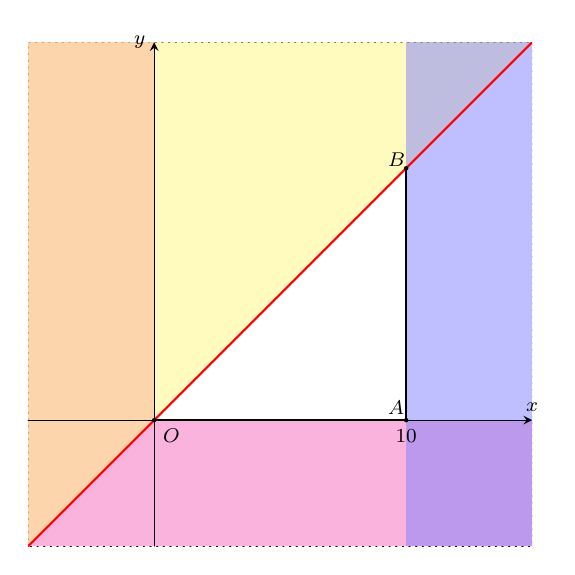
\begin{tikzpicture}[>=stealth,line join=round,line cap=round,font=\footnotesize,scale=.8,x=1cm,y=1cm,every node/.style={scale=0.9},declare function={
								m=-2;M=6;a=4;
								f(\x)=(\x);}
					]
					\begin{scope}
						\clip (m,m) rectangle (M,M);
						\draw[dotted] (m,m) rectangle (M,M);
						\fill[magenta!50,opacity=.6] (m,m) rectangle (M,0)
						(m,m) rectangle (0,M)
						;
						\fill[yellow!50,opacity=.5] plot[domain=m:M] (\x,{f(\x)})--(m,M)|-cycle;
						\fill[blue!50,opacity=.5] (a,m) rectangle (M,M);
						\draw[red,thick,samples=150,smooth,domain=m:M] plot(\x,{f(\x)});
						\draw[semithick] (0,0)--(a,0)node[below]{$10$}--(a,{f(a)});
					\end{scope}
					\draw[->] (m,0)--(M,0)node[above]{$x$};
					\draw[->] (0,m)--(0,M)node[left]{$y$};
					\fill (0,0)circle(1pt)node[below right]{$O$}
					(a,0)circle(1pt)+(130:0.25)node{$A$}
					(a,{f(a)})circle(1pt)+(140:0.2)node{$B$}
					;
				\end{tikzpicture}
			\end{center}
			Miền nghiệm của hệ bất phương trình là phần không tô màu ở hình trên. Khi đó tọa độ các điểm $O(0,0)$, $A(10,0)$ và $B(10,10)$.\\
			Và
			$f(0;0)=20(0+0)=0$; $f(10;0)=20(10+0)=200$; $f(10;10)=20(10+10)=400$.\\
			Do đó $f(x,y)=20(x+y)\leq 400$ nên suy ra $T\leq 20(x+y)\leq 400$.\\
			Do đó số tiền thu được tối đa là $400$ nghìn đồng.
		\end{itemchoice}
	}
\end{ex}

\Closesolutionfile{ans}

\begin{ex}%[H]giảng 10 New - 4in1, Nguyễn Vân Trường]%[0H4H1-2]
	Cho $\alpha$ thoả mãn $90^\circ<\alpha<180^\circ$ và $\sin\alpha=\dfrac{4}{5}$.
	\choiceTF[t]
	{\True $\cos\alpha<0$}
	{$\cos\alpha=\dfrac{2\sqrt{2}}{3}$}
	{$\cot\alpha=\dfrac{3}{4}$}
	{\True $P=3\tan \alpha - 2 \cot \alpha = -\dfrac{5}{2}$}
	\loigiai{

		\begin{itemchoice}
			\itemch Vì $90^\circ<\alpha<180^\circ$ nên
			nên $\cos\alpha<0$.
			\itemch Vì $\cos \alpha <0$ nên $\cos\alpha=-\sqrt{1-\sin^2\alpha}=-\dfrac{3}{5}$.
			\itemch Vì $\cot \alpha = \dfrac{\cos \alpha}{\sin \alpha} = -\dfrac{3}{5}: \dfrac{4}{5} =- \dfrac{3}{4}$.
			\itemch Vì $\tan \alpha = \dfrac{1}{\cot \alpha} =- \dfrac{4}{3}$ nên $P=3\tan \alpha - 2 \cot \alpha = 3\cdot \left(-\dfrac{4}{3}\right) - 2\cdot \left(-\dfrac{3}{4}\right) = -\dfrac{5}{2}$.
		\end{itemchoice}
	}
\end{ex}
% % \indapan{3}{ans-DS}

\caukq

\Opensolutionfile{ans}[ans-KQ]

\begin{ex}%[0D1V2-3]%[KNTT - Lớp 10 - Ôn tập giữa học kì 1 - Đề 1]%[Dương Văn Đức]
	Cho hai tập hợp $A=(m-1;8]$; $B=(2;16-m)$, $m\in \mathbb{R}$. Có bao nhiêu số nguyên $m$ để $A\setminus B=\varnothing$?
	\shortans{$5$}
	\loigiai{
	Điều kiện $\heva{&m-1<8\\&2<16-m}\Leftrightarrow\heva{&m<9\\&m<14}\Leftrightarrow m<9$.\\
	Để $A\setminus B=\varnothing \Leftrightarrow A\subset B\Leftrightarrow\heva{&m-1\geq 2\\&16-m>8}\Leftrightarrow\heva{&m\geq 3\\&m<8}\Leftrightarrow m\in[3;8)$.\\
	Vì $m$ nguyên nên $m \in \{3;4;5;6;7\}$. Vậy có $5$ số nguyên thỏa yêu cầu bài toán.
	}
\end{ex}

%%%%%-----Câu 20.-----%%%%%
\begin{ex}%[0H4V3-1]%[KNTT - Lớp 10 - Ôn tập giữa học kì 1 - Đề 1]%[Dương Văn Đức]
	Hai chiếc tàu thủy cùng xuất phát từ vị trí $A$, đi thẳng theo hai hướng hợp với nhau một góc $60^\circ$. Tàu thứ nhất chạy với tốc độ $35$ km/h, tàu thứ hai chạy với tốc độ $40$ km/h. Hỏi sau $2$ giờ hai tàu cách nhau bao nhiêu ki-lô-mét?
	\begin{center}
		\begin{tikzpicture}[scale=1, font=\footnotesize, line join=round, line cap=round, >=stealth,declare function={ac=3;ab=4;g=60;}]
			\path (0,0)coordinate(A)
			(ab,0)coordinate(B)
			(g:ac)coordinate(C)
			;
			\draw (C)--(A)--(B);
			\foreach \p\g in {A/-90,B/-90,C/-80}\fill (\p)circle(1pt)+(\g:0.25)node[scale=.8]{$\p$};
			\path pic[draw,angle radius = 10pt,angle eccentricity=1.7,"{\scriptsize $60^\circ$}"] {angle = B--A--C};
			\foreach \x in {1,2,3}
			\foreach \y in {0,1,2,3,4,5}
			\draw(0.25+\y,\x-0.25)--(\y,\x-0.25);
			\foreach \x in {1,2,3}
			\foreach \y in {0,1,2,3,4,5}
			\draw(-0.25+\y,\x-0.75)--(\y,\x-0.75);
			\fill plot [smooth cycle] coordinates{(3.75,0)(4.25,0)(4.3,0.2)(4.15,0.2)(4.15,0.3)(4.05,0.3)(4.05,0.4)(3.95,0.4)(3.95,0.3)(3.85,0.3)(3.85,0.2)(3.7,0.2)} ;
			\fill plot [smooth cycle] coordinates{(1.25,2.5)(1.75,2.5)(1.8,2.7)(1.65,2.7)(1.65,2.8)(1.55,2.8)(1.55,2.9)(1.45,2.9)(1.45,2.8)(1.35,2.8)(1.35,2.7)(1.2,2.7)} ;
		\end{tikzpicture}
	\end{center}
	\shortans{$75{,}5$}
	\loigiai{
		Vị trí tàu thủy thứ nhất và tàu thủy thứ hai sau $2$ giờ lần lượt ở vị trí $C$ và $B$.\\
		Do tàu thứ nhất chạy với tốc độ $35$ km/h nên $AC=35\cdot 2=70$.\\
		Do tàu thứ hai chạy với tốc độ $40$ km/h nên $AB=40\cdot 2=80$.\\
		Áp dụng định lý côsin vào $\triangle ABC$, ta có
		\begin{eqnarray*}
			& & BC^2=AB^2+AC^2-2AB\cdot AC\cdot \cos A\\
			&\Leftrightarrow & BC^2=70^2+80^2-2\cdot 70\cdot 80\cdot \cos 60^\circ=5700\\
			&\Rightarrow & BC\approx 75{,}5.
		\end{eqnarray*}
		Vậy sau $2$ giờ, hai tàu cách nhau khoảng $75{,}5$ km.
	}
\end{ex}
%%%%%-----Câu 21.-----%%%%%
\begin{ex}%[0D2C2-3]%[KNTT - Lớp 10 - Ôn tập giữa học kì 1 - Đề 1]%[Dương Văn Đức]
	Một xưởng sản xuất bàn và ghế. Một chiếc bàn cần $1{,}5$ giờ lắp ráp và $1$ giờ hoàn thiện; một chiếc ghế cần $1$ giờ lắp ráp và $2$ giờ hoàn thiện. Bộ phận lắp ráp có $3$ nhân công, bộ phận hoàn thiện có $4$ nhân công, một nhân công làm việc không quá $8$ tiếng mỗi ngày. Thị trường luôn tiêu thụ hết sản phẩm của xưởng và lượng ghế tiêu thụ không vượt quá $3{,}5$ lần số bàn. Biết một chiếc bàn lãi
	$600$ nghìn đồng, một chiếc ghế lãi $450$ nghìn đồng. Gọi $x$, $y$ lần lượt là số bàn, số ghế mà xưởng sản xuất trong một ngày để thu được tiền lãi cao nhất. Tính $10x+11y$.
	\shortans{$212$}
	\loigiai{
	Do $x$, $y$ lần lượt là số bàn, số ghế mà xưởng sản xuất trong một ngày ($x$, $y\in \mathbb{N}$).
	\begin{center}
		\begin{tikzpicture}[>=stealth,line join=round,line cap=round,font=\footnotesize,scale=.8,x=.25cm,y=.25cm,every node/.style={scale=0.9},declare function={
						m=-4;xmax=36;ymax=28;
						f(\x)=24-1.5*(\x);
						g(\x)=16-(\x)/2;
						h(\x)=3.5*(\x);
					}
			]
			\begin{scope}
				\clip (m,m) rectangle (xmax,ymax);
				\draw[dotted] (m,m) rectangle (xmax,ymax);
				\fill[pattern=horizontal lines] (m,m) rectangle (xmax,0)
				(m,m) rectangle (0,ymax);
				\draw[fill,pattern=north east lines,opacity=.5] plot[domain=m:xmax] (\x,{f(\x)})--(xmax,m)|-cycle;
				\draw[fill,pattern=north west lines,opacity=.5] plot[domain=m:xmax] (\x,{g(\x)})--(xmax,ymax)-|cycle;
				\draw[fill,pattern=north west lines,opacity=.5] plot[domain=m:xmax] (\x,{h(\x)})--(m,ymax)|-cycle;
			\end{scope}
			\draw[->] (m,0)--(xmax+0.1,0)node[above]{$x$};
			\draw[->] (0,m)--(0,ymax+0.1)node[left]{$y$};
			\fill (0,0)circle(1.5pt)node[above right]{$O$}
			;
			\foreach \i in {4,8,...,36}\draw (\i,2pt)--(\i,-2pt);
			\foreach \i in {4,8,...,28}\draw (2pt,\i)--(-2pt,\i);
			\path (4,14)+(-160:0.7)node[scale=0.8,fill=white,inner sep=0pt]{$A$}
			(8,12)+(80:0.7)node[scale=0.8,inner sep=0pt,fill=white]{$B$}
			(16,0)node[scale=0.8,below,fill=white,inner sep=0pt]{$16$}+(70:0.7)node[scale=0.8,inner sep=0pt,fill=white,,inner sep=0pt]{$C$}
			(32,0)node[scale=0.8,below,fill=white,inner sep=0pt]{$32$}
			(0,16)node[scale=0.8,left,fill=white,inner sep=0pt]{$16$}
			(0,24)node[scale=0.8,left,fill=white,inner sep=0pt]{$24$}
			;
		\end{tikzpicture}
	\end{center}
	Theo bài ra ta có hệ
	$\heva{&1{,}5x+y\leq 24\\&x+2y\leq 32\\&3{,}5x-y\geq 0\\&x\geq 0,\ y\geq 0.}$\\
	Miền nghiệm của hệ là miền tứ giác $OABC$ với $O(0;0)$, $A(4;14)$, $B(8;12)$, $C(16;0)$.\\
	Tiền lãi thu được là $F(x;y)=600x+450y$.\\
	Ta có
	\begin{itemize}
		\item $F(0;0)=600\cdot 0+450\cdot 0=0$.
		\item $F(4;14)=600\cdot 4+450\cdot 14=8700$.
		\item $F(8;12)=600\cdot 8+450\cdot 12=10200$.
		\item $F(16;0)=600\cdot 16+450\cdot 0=9600$.
	\end{itemize}
	$F$ đạt giá trị lớn nhất bằng $10\,200\,000$ đồng tại $(x;y)=(8;12)$.\\
	Để thu được tiền lãi cao nhất thì một ngày, xưởng sản xuất $8$ chiếc bàn và $12$ chiếc ghế. Khi đó tiền lãi mỗi ngày là $10\,200\,000$ đồng.\\
	Vậy $x=8,\ y=12 \Rightarrow 10x+11y=212$.}
\end{ex}

\begin{ex}%[BG - 10 New - 4in1,Nguyễn Văn Sang]%[0H4H2-2]
	Tính diện tích tam giác $ABC$, biết $AB=6$ và $2\sin A=3\sin B=4\sin C$, làm tròn đến hàng phần mười.
	\shortans{$42{,}7$}
	\loigiai{
		Theo định lý sin ta có $\dfrac{AB}{\sin C}=\dfrac{AC}{\sin B}=\dfrac{BC}{\sin A}=2R\Rightarrow \heva{&BC=2R\sin A\\ &AC=2R\sin B\\&AB=2R\sin C}$\\
		Từ $2\sin A=3\sin B=4\sin C\Leftrightarrow 2R \cdot 2\sin A= 2R \cdot 3\sin B=2R \cdot 4\sin C \Leftrightarrow 2BC=3AC=4AB$.\\
		Mà $AB=6$ nên $AC=8$, $BC=12$, suy ra nửa chu vi tam giác bằng $p=\dfrac{6+8+12}{2}=13$.\\
		Theo công thức Hê-rông ta có
		\[S_{ABC}=\sqrt{p(p-a)(p-b)(p-c)}=\sqrt{13(13-6)(13-8)(13-12)}=2\sqrt{455}\approx 42{,}7.\]
	}
\end{ex}
\Closesolutionfile{ans}

\TL
% % \indapan{6}{ans-KQ}
%%%%%-----Câu 19.-----%%%%%
\begin{ex}%[0H4C3-2]%[KNTT - Lớp 10 - Ôn tập giữa học kì 1 - Đề 1]%[Dương Văn Đức]
	Mặt tiền nhà ông An có chiều ngang $AB=4$ m, ông An muốn thiết kế lan can nhô ra có dạng là một phần của đường tròn $(C)$. Vì phía trước vướng cây tại vị trí $F$ nên để an toàn, ông An cho xây đường cong cách 1 m tính từ trung điểm $D$ của $AB$ (tức $ED=1$ m). Biết $AF=2$ m, $\widehat{DAF}=60^\circ$ và lan can cao $1$ m làm bằng inox với giá $2{,}2$ triệu/m$^2$. Tính số tiền ông An phải trả theo đơn vị triệu đồng (làm tròn kết quả tới hàng phần trăm).
	\begin{center}
		\begin{tikzpicture}[scale=1, font=\footnotesize, line join=round, line cap=round, >=stealth,declare function={R=3;g=40;}]
			\path (0,0)coordinate(O)
			(g:R)coordinate(B)
			(180-g:R)coordinate(A)
			($(A)!1/2!(B)$)coordinate (D)
			($(A)!1!60:(D)$) coordinate (F);
			;
			\draw[name path=df] (D)--(F);
			\draw[name path=circleO] (B)arc(g:180-g:R);
			\path[name intersections={of=df and circleO, by=E}];
			\pgfresetboundingbox
			\draw (F)--(A)--(B);
			\path pic[draw,angle radius = 10pt] {angle = D--A--F};
			\foreach \p\g in {A/180,B/0,D/-90,F/90,E/80}\fill(\p)circle(1pt)+(\g:0.25)node[scale=.8]{$\p$};
			\path (45+g/2:{1.1*R})node{$(C)$};
		\end{tikzpicture}
	\end{center}
	% \shortans{$9{,}99$}
	\loigiai{
		\begin{center}
			\begin{tikzpicture}[scale=1, font=\footnotesize, line join=round, line cap=round, >=stealth,declare function={R=3;g=40;}]
				\path (0,0)coordinate(O)
				(g:R)coordinate(B)
				(180-g:R)coordinate(A)
				($(A)!1/2!(B)$)coordinate (D)
				($(A)!1!60:(D)$) coordinate (F);
				;
				\draw[name path=df] (D)--(F);
				\draw[name path=circleO] (B)arc(g:180-g:R);
				\path[name intersections={of=df and circleO, by=E}];
				\draw (F)--(A)--(O)--(B)--(A)--(E)--(B);
				\path pic[draw,angle radius = 10pt] {angle = D--A--F};
				\foreach \p\g in {A/180,B/0,D/-90,F/90,E/80,O/-90}\fill(\p)circle(1pt)+(\g:0.25)node[scale=.8]{$\p$};
				\path (45+g/2:{1.1*R})node{$(C)$};
			\end{tikzpicture}
		\end{center}
		Theo giả thiết, ta có $AF=AD=2$ và $\widehat{DAF}=60^\circ$ nên $\triangle AFD$ đều.\\
		Vì $ED=1$ nên $AE$ vừa là trung tuyến, vừa là phân giác. Nên $\widehat{EAD}=30^\circ$ và $\widehat{EDB}=180^\circ - \widehat{EDA}=120^\circ$.\\
		Trong $\triangle EDB$ có $EB^2=DE^2+DB^2-2DE\cdot DB\cdot \cos 120^\circ=7 \Rightarrow EB=\sqrt{7}$.\\
		Gọi $R$ là bán kính của đường tròn $(C)$ tâm $O$.\\
		Áp dụng định lý sin trong tam giác $\triangle AEB$ ta có $2R=\dfrac{EB}{\sin \widehat{EAD}}=\dfrac{\sqrt{7}}{\sin 30^\circ}$. Suy ra $R=\sqrt{7}$.\\
		Xét tam giác $OAB$ có $R=OA=OB=\sqrt{7}$, $AB=4$.\\
		Suy ra $\cos \widehat{AOB}=\dfrac{OA^2+OB^2-AB^2}{2OA\cdot OB}=-\dfrac{1}{7}\Rightarrow\widehat{AOB}\approx 98{,}21^\circ$.\\
		Suy ra độ dài cung nhỏ $AB$ là $l=\dfrac{98{,}21}{180}\cdot \pi\cdot R\approx 4{,}54$ (m).\\
		Vì chiều cao của lan can là $1$ m và giá kính là $2{,}2$ triệu/m$^2$ nên số tiền ông An phải trả là
		$4{,}54\cdot 1\cdot2{,2}\approx 9{,}98 \;\text{(triệu đồng).}$
	}
\end{ex}
%%%%%-----Câu 22.-----%%%%%
\begin{ex}%[0D1V3-5]%[KNTT - Lớp 10 - Ôn tập giữa học kì 1 - Đề 1]%[Dương Văn Đức]
	Khối $10$ của một trường THPT có $440$ em học sinh, trong đó có $250$ em thích môn Văn, $210$ em thích môn Toán, $240$ em thích môn Anh, $65$ em không thích môn nào, $75$ em thích cả ba môn. Hỏi số em chỉ thích một trong ba môn trên là bao nhiêu?
	% \shortans{$125$}		
	\loigiai{
		Gọi $a$, $b$, $c$ theo thứ tự là số học sinh chỉ thích Văn, Toán, Anh.\\
		$x$ là số học sinh chỉ thích hai môn Văn, Toán;\\
		$y$ là số học sinh chỉ thích hai môn Anh, Toán;\\
		$z$ là số học sinh chỉ thích hai môn Văn, Anh.\\
		Điều kiện $a$, $b$, $c$, $x$, $y$, $z\in \mathbb{N}$.\\
		\begin{center}
			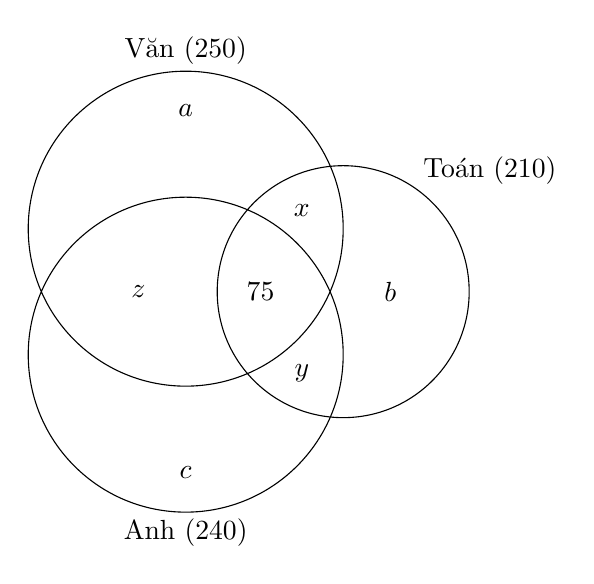
\begin{tikzpicture}
				\def\d{0.8} \def\r{2}
				\def\firstE{(90:\d) circle (\r)}
				\def\secondE{(-90:\d)circle (\r)}
				\def\thirdE{(0:2.5*\d)circle ({0.8*\r})}
				\draw \firstE
				\secondE
				\thirdE
				;
				\path (15:2*\r) node[above=2mm] {Toán ($210$)}
				(90:2.2*\d) node[above=10mm] {Văn ($250$)}
				(-90:2.2*\d) node[below=10mm]  {Anh ($240$)}
				(0.95,0)node{$75$}
				(90:1.15*\r)node{$a$}
				(0:1.3*\r)node{$b$}
				(-90:1.15*\r)node{$c$}
				(35:0.9*\r)node{$x$}
				(-35:.9*\r)node{$y$}
				(180:0.3*\r)node{$z$}
				;
			\end{tikzpicture}
		\end{center}
		Số học sinh thích ít nhất 1 trong ba môn là $440-65=375$.\\
		Ta có hệ phương trình
		\begin{eqnarray*}
			\heva{&a+x+z+75=250&(1)\\&b+x+y+75=210&(2)\\&c+y+z+75=240&(3)\\&a+b+c+x+y+z+75=375&(4)}
		\end{eqnarray*}
		Cộng (1), (2), (3) vế theo vế ta được $a+b+c+2(x+y+z)=475$.\tagEX{5}\noindent
		Từ (4), (5) suy ra $a+b+c=125$.\\
		Vậy có $125$ học sinh chỉ thích một trong ba môn Toán, Anh, Văn.
	}
\end{ex}
% \newpage .